\thispagestyle{empty}

\begin{center}
  \theauthor
\end{center}

\medskip
\begin{center}
  \textbf{\MakeUppercase{\thetitle}}
\end{center}

\medskip
\noindent {\small Este Trabalho de Conclusão de Curso foi julgado adequado no contexto da disciplina EEL7890 - Trabalho de conclusão de Curso (TCC), e aprovado em sua forma final pelo Departamento de Engenharia Elétrica e Eletrônica da Universidade Federal de Santa Catarina.}

\begin{center}
  Florianópolis, \thedate.
\end{center}

\medskip
\begin{center}
  \textbf{Banca examinadora:}
\end{center}
\bigskip

% Versão pra impressão (sem assinaturas)
 
\begin{center}
  %\rule{60mm}{0.2mm}\\
  
\includegraphics[width=60mm]{signatures/danilo}\\
  Prof.\ \theadvisor, Ph.D.\\
  {\footnotesize Universidade Federal de Santa Catarina}
\end{center}
\bigskip
\begin{center}
  %\rule{60mm}{0.2mm}\\
  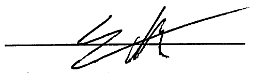
\includegraphics[width=60mm]{signatures/eduardo}\\
  Prof. Eduardo Batista, Dr.\\
  {\footnotesize Universidade Federal de Santa Catarina}
\end{center}
\bigskip
\begin{center}
  %\rule{60mm}{0.2mm}\\
  
\includegraphics[width=60mm]{signatures/marcio}\\
  Prof. Marcio Costa, Dr.\\
  {\footnotesize Universidade Federal de Santa Catarina}
\end{center}

% Imprimir em formato A5, após scanear usar algum editor de imagens apenas para assinaturas, como exemplo a figura assinaturas.png

%\begin{center}
%	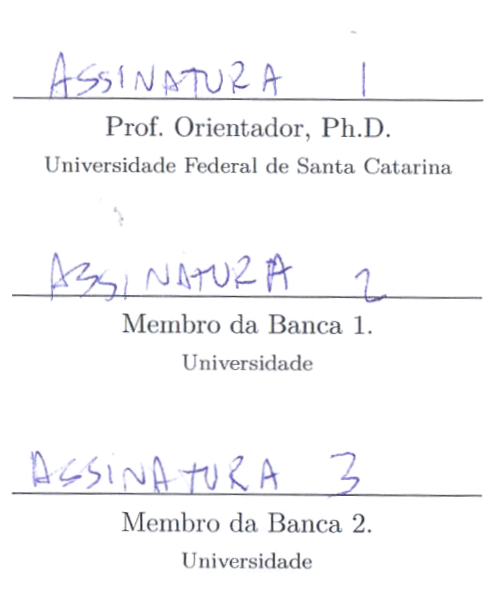
\includegraphics{assinaturas}
%\end{center}

% Para melhor qualidade scanear (ou então após usar algum editor de imagens) cada assinatura separadamente, como exemplo a Figura assinatura01.png

%\begin{center}
%	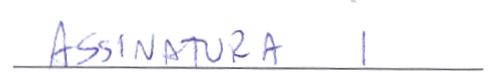
\includegraphics{assinatura01}\\
%	Prof.\ \theadvisor, Ph.D.\\
%	{\footnotesize Universidade Federal de Santa Catarina}
%\end{center}
%\bigskip
%\begin{center}
%	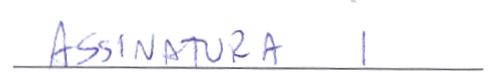
\includegraphics{assinatura01}\\
%	Membro da Banca 1.\\
%	{\footnotesize Universidade}
%\end{center}
%\bigskip
%\begin{center}
%	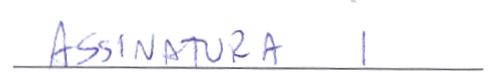
\includegraphics{assinatura01}\\
%	Membro da Banca 2.\\
%	{\footnotesize Universidade}
%\end{center}

\medskip


\cleardoublepageempty
